We are now ready to perform the experiments. We will begin exploring SimCLR implementation and results, later we will explore BYOL's implementation and lastly we will compare them in order to see how BYOL tries to improve SimCLR and we will check if it successess or not.

The code used for the experimentations, as well as some files with the results, can be found on the Github repository for this work.

\section{SimCLR exploration}
We will perform an iterative exploration with this framework. We will explore a few range for a subset of the hyperparameters and then we will go deeper into some hyperparameters to try and obtain better results.

\subsection{First approach}
\label{experiments:simclr:first}

The first thing we did to experiment with this framework is to explore a wide range of hyperparameters to see which set of them performed better for us. The script that can be found in \lstinline{code/SimCLR/run.py}.

What we did for this first exploration was to define a \emph{parameter grid} and execute the whole framework using each combination of the parameters. The parameters that were firstly considerered are:
\begin{enumerate}
\item \lstinline{batch_size}. This is one of the most important parameters of SimCLR. In the original paper, it was proven that the higher this parameter, the better the results obtained for the linear classification. This parameter is also important since it has to adapt to our GPU's memory. The options that we have considered for the first experiments are: \lstinline|batch_size = {512,1024}|.

\item \lstinline{temperature}. The temperature parameter $\tau$ plays an important role in the individual loss seen in Equation \eqref{c:loss:simclr:ind}. It is suggested to try values in the range $[0,1]$ and the one that had better performance for the original experiments was around $0.5$, so we chose the following values: \lstinline|temperature = {0.25,0.5,0.75,1}|.

\item \lstinline{color_jitter_strength}. This parameter measures how hard is the color variation in the data augmentation. Previous results show that this parameter is important for the success of the network, so we provide with a big range of values. We include the following values: \lstinline|color_jitter_strength = {0.25,0.5,0.75,1}|.
\end{enumerate}

Using python and the python function \lstinline{itertools.product} we straightforwardly generate all possible different combinations of unions of the parameters so we only have to append them to a general string and execute the \lstinline{run.py} script mentioned before to obtain the results. In total, we obtain $32$ possible combinations, so we will obtain $32$ models. 

The script was executed and took approximately $24$ hours to train and evaluate all different models, obtaining the results in Table \ref{table:experiment:first:simclr} in Appendix \ref{APPENDIX:B}. We have to remark, for each of the two possible batch sizes, the best results obtained. These are:

\begin{table}[H]
    \label{table:best:first:simclr}
\centering
\resizebox{\columnwidth}{!}{
\begin{tabular}{rrrrrrr}
batch\_size   & temperature   & color\_jitter & regularization\_loss & top\_1\_accuracy & top\_5\_accuracy & steps         \\ \hline
 512  &  0.25 &  0.25 &  0.0093      &  0.833         &  0.994          &  9800 \\
 1024 &    0.25       &  0.75 &  0.0093      &  \textbf{0.841}          &  0.995          &  4900 \\
\end{tabular}
}
\caption{Best results for the grid search experiment with SimCLR.}
\end{table}

Let us make some observations. The clearest is that, since the second batch size doubles the first one, the training ends in half the steps. We can see that the temperature obtained in both cases is the same, and it is equal to $0.25$. However, there is a big change in the color jitter parameter: while using $512$ as batch size obtains the best result with the value of $0.25$ for color jitter, using $1024$ as batch size this value changes to $0.75$, which implies stronger color changes on the data augmentation. 

Although both models get to the same value of regularization loss, the model with a batch size of $1024$ obteins a higher \emph{top 1 accuracy}.

\begin{figure}[htp] 
    \centering
    \subfloat[Tulips]{%
        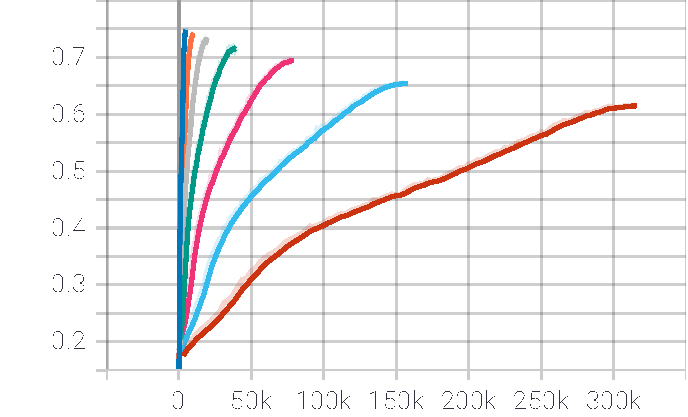
\includegraphics[width=0.45\textwidth]{train_supervised_acc}%
        \label{fig:accs:}%
        }%
    \hfill%
    \subfloat[Rotated, flipped tulips]{%
        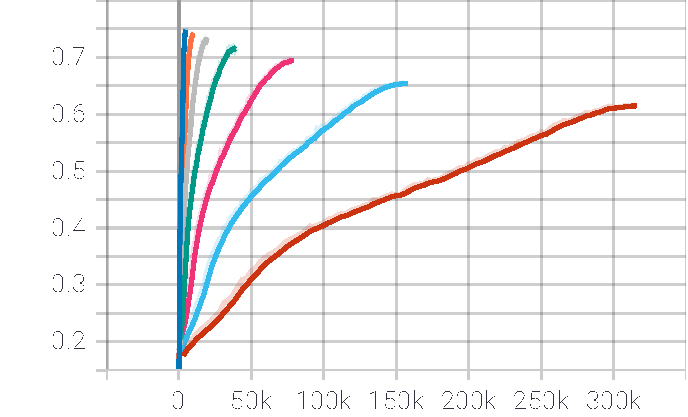
\includegraphics[width=0.45\textwidth]{train_supervised_acc}%
        \label{fig:rot:flip:flowers}%
        }%
        \caption{The image on the left is the original image, and the image on the right is a new example generated by first a rotation of a random angle and then a flip.}
\end{figure}